\chapter{Soluciones circulares a las ecuaciones de movimiento}
\label{cap:4}
\newpage

\section{Planteamiento de las ecuaciones}

En \cite{Costa-Natario-Zilhao} observan casos particulares a las ecuaciones de movimiento mostradas en \eqref{eq:66}, concretamente se estudia como la ecuación \eqref{eq:66}, asumiendo la condición suplementaria de Pirani, se reduce a 
\begin{equation}
\label{eq:69}
\cd{p^{\mu}} = 0,
\end{equation}
considerando una 4-velocidad tal que $u^{\theta}=0$, y 
\begin{equation}
\label{eq:68}
\omega := \dv{\phi}{t} = \frac{a}{a^2 + R^2},
\end{equation}
donde $\omega$ es la velocidad angular para la cual los observadores miden un campo gravito-magnético nulo. Dicho análisis surge como análogo a un estudio realizado en el caso electromagnético, donde se obtienen las componentes no-nulas del tensor de marea magnético que, a diferencia del caso gravitacional, no puede ser reducido a \eqref{eq:69} ya que la parte antisimétrica de \eqref{eq:51} no puede ser nulo al considerar efectos de inducción electromagnética dentro del estudio.

Esto nos lleva a la pregunta si existen geodésicas tales que las condiciones anteriormente mencionadas. Las más simples de estudiar son las geodésicas circulares, es decir cuando además $u^r=0$. Sin embargo, es posible demostrar que no existen geodésicas circulares con velocidades angulares igual a \eqref{eq:68}, esto se puede ver al comparar \eqref{eq:68} con la velocidad angular de una geodésica circular (\textit{e.g.} \cite{Matolcsi})
\begin{equation}
\omega_{\mathrm{geo}} = \frac{1}{a + \sqrt{\frac{r^3}{M}}},
\end{equation}
de donde se deduce que el radio de la órbita debiera ser tal que se ésta encontraría al interior del horizonte de eventos del agujero negro.

Sin embargo, y pese al análisis anterior, aun existe una interrogante sobre \eqref{eq:69} que es, ¿existen soluciones circulares a \eqref{eq:69}? (ver figura \ref{fig:7}).
\begin{figure}[!h]
\centering
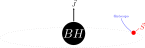
\includegraphics[scale=0.9]{images/solucion-en-kerr.pdf}
\caption[Solución helicoidal en Kerr]{Representación esquemática del sistema agujero negro-dipolo.}
\label{fig:7}
\end{figure}

Para responder esta pregunta procederemos a resolver las ecuaciones de movimiento \eqref{eq:69} y \eqref{eq:103}. Como estamos considerando órbitas circulares, y si por simplicidad suponemos que se encuentra en el plano ecuatorial, la velocidad de un observador co-móvil con el satélite es $u^{\mu} = \left[ u^t,0,0,u^{\phi} \right]$.

De \eqref{eq:68}, y la condición de normalización $u^{\mu}u_{\nu} = 1$, se obtiene que la 4-velocidad del satélite es
\begin{equation}
\label{eq:70}
u^{\mu} = \left [ \frac{\left(a^{2} + r^{2}\right)}{r\sqrt{a^{2} - 2 m r + r^{2}}}, \quad 0, \quad 0, \quad \frac{a}{r\sqrt{a^{2} - 2 m r + r^{2}}}\right ],
\end{equation}
y, definiendo $u_{\mu} := g_{\mu \nu} u^{\nu}$ tenemos que
\begin{equation}
\label{eq:71}
u_{\mu} = \left [ \frac{1}{r}\sqrt{a^{2} - 2 m r + r^{2}}, \quad 0, \quad 0, \quad -\frac{a}{r} \sqrt{a^{2} - 2 m r + r^{2}} \right ]
\end{equation}

Por otro lado, si definimos implícitamente el 4-vector de espín $S^{\mu}$ como 
\begin{equation}
S^{\mu} := -\frac{1}{2} \epsilon^{\mu \nu \rho \sigma} S_{\nu \rho} u_{\sigma},
\end{equation}
y tal que
\begin{equation}
S^{\mu \nu} = \epsilon^{\mu \nu \rho \sigma} S_{\rho} u_{\sigma},
\end{equation}
las ecuaciones de evolución para el vector de espín son
\begin{equation}
\label{eq:72}
\cd{S^{\mu}} = -S_{\nu} \cd{u^{\nu}} u^{\mu}.
\end{equation}

Reemplazando \eqref{eq:70} y \eqref{eq:71} en \eqref{eq:69} y \eqref{eq:72} se deducen las siguientes ecuaciones de movimiento para el momentum y el espín:
\begin{align}
\dot{p}^t(s) &= -\frac{m(R^2-a^2)}{R(a^2-2mR+R^2)^{3/2}} p^R(s),\\
\nonumber
\dot{p}^r(s) &= -\frac{\sqrt{a^2-2mR+R^2}}{R^5} \left( -a^{2}m p^t(s) - a m \left(a^{2} + R^{2}\right) p^{\phi}(s) + a \left(a^{2} m - R^{3}\right) p^{\phi}(s) \right.\\
& \quad \left. + m \left(a^{2} + R^{2} \right) p^t(s) \right),\\
\dot{p}^{\theta}(s) &= 0,\\
\dot{p}^{\phi}(s) &= -\frac{a(R-m)}{R(a^2-2mR+R^2)^{3/2}} p^r(s),\\
\dot{S}^t(s) &= -\frac{a^2}{R^2 \sqrt{a^2-2mR + R^2}} S^r(s),\\
\nonumber
\dot{S}^r(s) &= -\frac{\sqrt{a^2-2mR+R^2}}{R^5} \left( - a^{2} m S^t(s) - a m \left(a^{2} + R^{2}\right) S^{\phi}(s) + a \left(a^{2} m - R^{3}\right) S^{\phi}(s) \right.\\
& \quad \left. + m \left(a^{2} + R^{2} \right) S^t(s) \right),\\
\dot{S}^{\theta}(s) &= 0,\\
\dot{S}^{\phi}(s) &= \frac{a}{R\sqrt{a^2-2mR+R^2}} S^r(s).
\end{align} 

Las cuales son dos conjuntos de 4 ecuaciones ordinarias acopladas.

\section{Soluciones}

Luego de resolver las ecuaciones analíticamente, tenemos que la forma general de la solución es, para el caso del momentum, de la forma
\begin{align}
p^t(s) &= C_1 \alpha + \beta \left( C_2 e^{s \gamma} + C_3 e^{-s \gamma} \right),\\
p^r(s) &= \delta \left( C_2 e^{s \epsilon} - C_3 e^{-s \epsilon} \right),\\
p^{\theta}(s) &= C_4,\\
p^{\phi}(s) &= C_1 + C_2 e^{s \epsilon} + C_3 e^{-s \epsilon},
\end{align}
y para el espín es de la forma
\begin{align}
S^t(s) &= C_5 \eta + \kappa \left[ C_6 \cos\left(\frac{as}{R^2} \right) + C_7 \sin\left(\frac{as}{R^2} \right) \right],\\
S^r(s) &= C_6 \left[ \tau \sin\left(\frac{as}{R^2} \right) - \sigma \cos\left(\frac{as}{R^2} \right) \right] 
+ C_7 \left[ \tau \cos\left(\frac{as}{R^2} \right) - \sigma \sin\left(\frac{as}{R^2} \right) \right],\\
S^{\theta}(s) &= C_8,\\
S^{\phi}(s) &= C_5 + C_6 \cos\left(\frac{as}{R^2} \right) + C_7 \sin\left(\frac{as}{R^2} \right),
\end{align}
donde todos los elementos con letras griegas son factores que dependen de $(a,m,R)$ y no jugarán un rol importante en el futuro. Por otro lado, los coeficientes $C_1, \dots, C_8$ son constantes de integración y pueden ser calculadas reemplazando la solución en las condiciones que debe satisfacer.

La primera condición que imponemos es el hecho que al 4-velocidad y el 4-vector de espín deben ser ortogonales. De esta forma encontramos que $C_5=0$.

De \eqref{eq:44} y \eqref{eq:42} encontramos que las soluciones para el momentum y el espín deben estar relacionadas de forma que
\begin{equation}
p^{\mu} = M u^{\mu} + \epsilon^{\mu \nu \alpha \beta} \Gamma^{\rho}_{\nu \sigma} u_{\rho} u_{\alpha} S_{\beta} u^{\sigma},
\end{equation}
al reemplazar $\mu=r$ y $\mu=\theta$ se determina que $C_2 = C_3 = C_6 = C_7 = 0$, teniendo así que la forma general de las soluciones se reduce a 
\begin{align}
\label{eq:73}
p^{\mu} &= \left[ p^{\phi} \frac{a(m+R)}{m}, 0, 0, p^{\phi} \right],\\
\label{eq:74}
S^{\mu} &= \left[ 0,0,S^{\theta},0 \right],
\end{align}
donde se han renombrado las constantes $C_1$ y $C_4$ por $p^{\phi}$ y $S^{\theta}$ respectivamente.

Finalmente, reemplazando $\mu=t$ y $\mu=\phi$ se obtiene un sistema de dos ecuaciones lineales y dos incógnitas
\begin{align}
\frac{a p^{\phi}(m+R)}{m} &= \frac{S^{\theta} a^{3}}{R^{2} \sqrt{a^{2} - 2 m R + R^{2}}} - \frac{S^{\theta} a m}{R\sqrt{a^{2} - 2 m R + R^{2}}} + \frac{a^{3} p^{\phi}}{m R} + \frac{a p^{\phi} R}{m},\\
p^{\phi} &= \frac{S^{\theta} a^{2}}{R^{2}\sqrt{a^{2} - 2 m R + R^{2}}} - \frac{S^{\theta} m}{R\sqrt{a^{2} - 2 m R + R^{2}}} + \frac{a^{2} p^{\phi}}{m R}.
\end{align}

Dicho sistema es a un sistema compatible indeterminado, es decir, admite un conjunto infinito de soluciones descritas por
\begin{equation}
\label{eq:75}
S^{\theta} = - \frac{p^{\phi}R \sqrt{a^2 - 2mR +R^2}}{m}.
\end{equation}

Reemplazando \eqref{eq:75} en \eqref{eq:73} y \eqref{eq:74} encontramos que la solución exacta a las ecuaciones puede escribirse en términos de $p^{\phi}$ como
\begin{align}
p^{\mu} &= \left[ p^{\phi} \frac{a(m+r)}{m},\quad 0,\quad 0,\quad p^{\phi} \right],\\
S^{\mu} &= \left[0,\quad 0,\quad -\frac{p^{\phi} \sqrt{a^2+r^2-2mr}}{mr},\quad 0\right],
\end{align}
o, en términos de $S^{\theta}$, como
\begin{align}
\label{eq:76}
p^{\mu} &= \left [ - \frac{S^{\theta} a \left(m + r\right)}{r \sqrt{a^{2} - 2 m r + r^{2}} }, \quad 0, \quad 0, \quad - \frac{S^{\theta} m}{r\sqrt{a^{2} - 2 m r + r^{2}}}\right ],\\
\label{eq:77}
S^{\mu} &= \left [ 0, \quad 0, \quad S^{\theta}, \quad 0\right ].
\end{align}

Es importante destacar que la masa del satélite puede calcularse como
\begin{equation}
\label{eq:78}
M := p^{\mu} u_{\mu} = -\frac{S^{\theta}a}{r},
\end{equation}
y en términos de $M$, la solución puede escribirse como
\begin{align}
\label{eq:86}
p^{\mu} &= \left [ \frac{M \left(m + r\right)}{\sqrt{a^{2} - 2 m r + r^{2}}}, \quad 0, \quad 0, \quad \frac{M m}{a \sqrt{a^{2} - 2 m r + r^{2}}}\right ],\\
\label{eq:87}
S^{\mu} &= \left [ 0, \quad 0, \quad - \frac{Mr}{a}, \quad 0\right ].
\end{align}

\section{Propiedades de la solución}

De la solución podemos destacar varios puntos:
\begin{itemize}
\item[-] Los parámetros de la solución determinan una relación entre la masa y el espín del satélite, dicha relación nos da a entender que, por ejemplo, una vez fijado el valor del espín inmediatamente queda determinado el valor de la masa del satélite (o viceversa), de tal forma que se logre contrarrestar la atracción del agujero negro tal que la órbita se mantenga circular.
\item[-] La única dirección y sentido permitidos para el espín es ser antiparalelo a la rotación del agujero negro, esto es por el signo $-$ en \eqref{eq:78} que nos indica que el momento angular intrínseco del satélite debe ser opuesto a la rotación del agujero negro y el hecho de que la única componente no-nula para el espín es la componente $S^{\theta}$.
\end{itemize}

Es importante destacar que no es posible obtener el caso en la métrica de Schwarszchild a partir del resultado encontrado. Esto es por la suposición inicial al momento de plantear las ecuaciones de movimiento es que la velocidad angular del satélite es proporcional al parámetro rotacional del agujero negro, es decir $\omega \propto a$, y calcular el límite $a \rightarrow 0$ implica que $\omega = 0$, lo cual implicaría que la órbita no sería circular.

No obstante, es interesante hacer notar que si definimos la 4-fuerza sobre el satélite como
\begin{equation}
\label{eq:124}
F^{\mu} := M \cd{u^{\mu}} = \left[ 0, \frac{M(mR-a^2)}{R^3},0,0 \right],
\end{equation}
y si consideramos el caso asintótico, es decir $R \gg m $, entonces se puede deducir la ley de gravitación universal de Newton, esto cumple con el principio de correspondencia puesto que al encontrarse lejos del agujero negro no hay diferencia entre un agujero negro rotante y el campo gravitacional generado por una distribución de masa. Además, al ser una órbita circular en donde la único agente externo acutuando sobre el satélite tiene solo componente radial no-nula se puede ver que el satélite presenta un movimiento circular uniforme, ya que presenta una velocidad angular constante, logrando identificar así que \eqref{eq:124} corresponde a la fuerza centrípeta de la órbita.

Por último, es necesario agregar que la velocidad coordenada tangencial de la órbita es
\begin{equation}
v = \omega R = \frac{aR}{a^2 + R^2},
\end{equation}
lo cual en el mismo límite asintótico se reduce a
\begin{equation}
\label{eq:79}
v \approx \frac{a}{R},
\end{equation}
y reemplazando en \eqref{eq:78} se tiene que
\begin{align}
\nonumber
R &= -\frac{S^{\theta}a}{M},\\
\nonumber
&= -\frac{S^{\theta}aR}{MR},\\
\label{eq:80}
&= -\frac{vS}{M},
\end{align}
donde $S = R S^{\theta}$ y es el módulo del espín (que coincide con el valor de la componente $z$ en un plano cartesiano).

Podemos agregar que \eqref{eq:80} representa la misma condición encontrada en \cite{Costa-Herdeiro-Natario-Zilhao} para el problema análogo en el espaciotiempo de Minkowski en coordenadas cartesianas mostrando así que la solución obtenida en \eqref{eq:86} y \eqref{eq:87} se reduce asintóticamente al caso en la métrica plana.